\documentclass[11pt]{article}

\usepackage{graphicx}
%\usepackage{algorithmic}
%\usepackage{algorithm}
\usepackage{amssymb}
\usepackage{amsmath}
\usepackage{enumerate}
\usepackage[mathscr]{euscript}

\begin{document}

\pagenumbering{arabic}

\begin{center}
{\LARGE{\textbf{Affective Computing}}} \\
\Large\textsc{Ph.D. Comprehensive Exam} \\[1em]
\large\textnormal{Mohammad Shayganfar - mshayganfar@wpi.edu} \\
\large\textnormal{May, 26 2015}
\end{center}

\section{Introduction to Affective Computing}

In this section, I discuss the concept of artificial emotions. I briefly review
the influential cognitive theories which describe emotions. These theories
provide cognitive structure of emotions and some of them describe the underlying
evaluative processes of emotion eliciting mechanisms. This is important in my
work because I am interested to investigate how emotions are involved in
collaboration and how the dynamics of a collaboration structure impact the
underlying processes of emotion.

Studies show that the decision making of
humans is not always logical \cite{GrossbergGutowski:affect-cognition}, and in
fact, not only is pure logic not enough to model human intelligence, but it also
shows failures when applied in artificial intelligence systems
\cite{dreyfus:artificial-critique}. Emotions impact fundamental parts of
cognition including perception, memory, attention and reasoning
\cite{clore:judgement-regulation}. This impact is caused by the information
emotions carry about the environment and event values. The influence of emotions
depends on an individual's focus of attention. For instance, a positive affect
can cause a positive attitude towards an object if the individual's focus is on
the object, whereas the same positive affect can be interpreted as a positive
feedback towards one's partner during the course of a collaboration. As another
example, a positive feedback can promote certain cognitive processes, or it can
inhibit other cognitive processes according to the conditions in the environment
\cite{clore:affective-guidance}. In both cases, emotions play a regulatory role
for cognitive processes \cite{gross:emotion-generation-regulation}. Some of the
effects flow from underlying shifts in the way people perceive and think under
the influence of emotion.

\section{Computational Theories of Emotion/Affect}

There are different types of computational theories of emotion. These theories
differ in type of relationships between their components and whether a
particular component play a cricual role in an individual emotion. For instance,
the basic component of an emotion can be the behavioral tendencies, cognitive
elements, or somatic processes. Emotion theories can also differ based on their
representationial distinction.

\subsection{Appraisal Theory}
\label{sec:appraisal-theory}

Appraisal theories of emotion were first formulated by Arnold
\cite{arnold:emotion-personality} and Lazarus \cite{lazarus:emotion-adaptation}
and then were actively developed in the early 80s by Ellsworth and Scherer and
their students \cite{roseman:appraisal-theory}
\cite{sander:systems-approach-appraisal} \cite{scherer:nature-function-emotion}
\cite{scherer:appraisal-processes} \cite{scherer:emotions-emergent}. The
emotional experience is the experience of a particular situation
\cite{frijda:emotions}. Appraisal theory describes the cognitive process by
which an individual evaluates the situation in the environment with respect to
the individual's well-being and triggers emotions to control internal changes
and external actions.

\begin{figure}[tbh]
  \center
  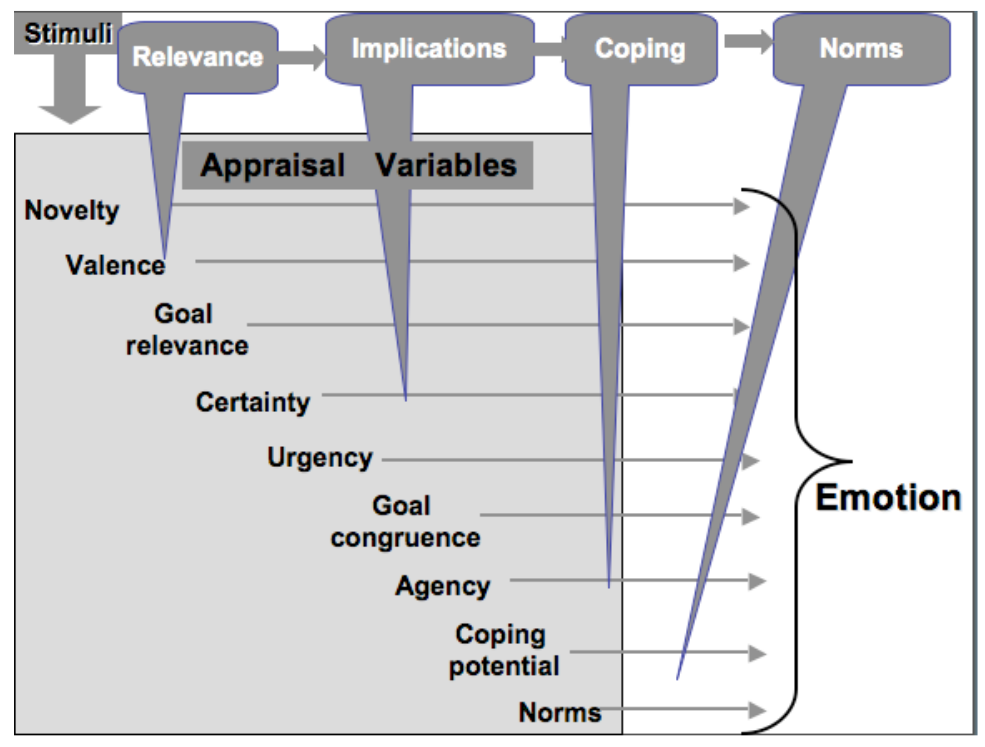
\includegraphics[width=0.8\textwidth]{figure/cpm.png}
  \caption{Schematic View of the Componential Theory of Emotion
  \cite{hudlicka:guidelines-emotions}.}
  \label{fig:cpm}
\end{figure}

\subsubsection{Componential approach}
\label{sec:componential-theories}

This approach emphasizes the distinct components of emotions, and is often
called the \textit{componential} appraoch \cite{leventhal:emotion-cognition}.
The ``components" referred to in this approach are the components of the
cognitive appraisal process. These are referred to as \textit{appraisal
variables}, and include \textit{novelty, valence, goal relevance, goal
congruence}, and \textit{coping abilities}
(further on, in this section, some of the appraisal variables used in
computational models are introduced)
\cite{scherer:nature-function-emotion,scherer:appraisal-processes}. A stimulus,
whether real or imagined, is analyzed in terms of its meaning and consequences
for the agent, to determine the affective reaction. The analysis involves
assigning specific values to the appraisal variables. Once the appraisal
variable values are determined by the organism’s evaluative processes, the
resulting vector is mapped onto a particular emotion, within the n-dimensional
space defined by the n appraisal variables. The semantic primitives for
representing emotions within this model are thus these individual appraisal
variables. Figure \ref{fig:cpm} shows the relationship of the individual
appraisal dimensions to the broader categories of evaluations taking place
during appraisal (Relevance, Implications, etc.).

\subsubsection{Component Process Model}
\label{sec:cpm}

The Component Process Model (CPM) is Scherer's influential and major theory of
emotions
\cite{scherer:sequential-appraisal-process,scherer:appraisal-processes}. This
theory focuses on the dynamic unfolding of emotions. The CPM suggests that an
event and its consequences are appraised with a set of criteria on multiple
levels of processing (the appraisal component). The result of the appraisal will
generally have a motivational effect, often changing or modifying the
motivational state before the occurrence of the event. Based on the appraisal
results and the motivational changes, some effects will occur in the autonomic
and somatic nervous system. The CPM considers emotions as the synchronisation of
many different cognitive and physiological components. Emotions are identified
with the overall process whereby low level cognitive appraisals, in particular
the processing of relevance, trigger bodily reactions, behaviours and subjective
feelings. The model suggests that there are four major appraisal objectives to
adaptively react to a salient event \cite{scherer:dynamic-architecture-emotion}: 

\begin{enumerate}[a)]
  \item \textbf{Relevance:} How relevant is this event for the agent? Does it
  directly affect the agent or its social reference group?
  \item \textbf{Implications:} What are the implications or consequences of this
  event and how do they affect agent's well-being and its immediate or long-term
  goals?
  \item \textbf{Coping Potential:} How well can the agent cope with or adjust to
  these consequences?
  \item \textbf{Normative Significance:} What is the significance of this event
  for the agent's self-concept and for social norms and values?
\end{enumerate}

To attain these objectives, the agent evaluates the event and its consequences
on a number of criteria or \textit{Stimulus Evaluation Checks} (SECs), with the
results reflecting the agent’s subjective assessment of consequences and
implications on a background of personal needs, goals, and values
\cite{scherer:appraisal-processes}. Figure \ref{fig:comp-cpm} shows the
postulated sequence, the cognitive and motivational inputs and the effects on
response systems. Also, the bidirectional effects between appraisal and other
cognitive functions are illustrated by the arrows in the upper part of Figure
\ref{fig:comp-cpm}.

\begin{figure}[tbh]
  \center
  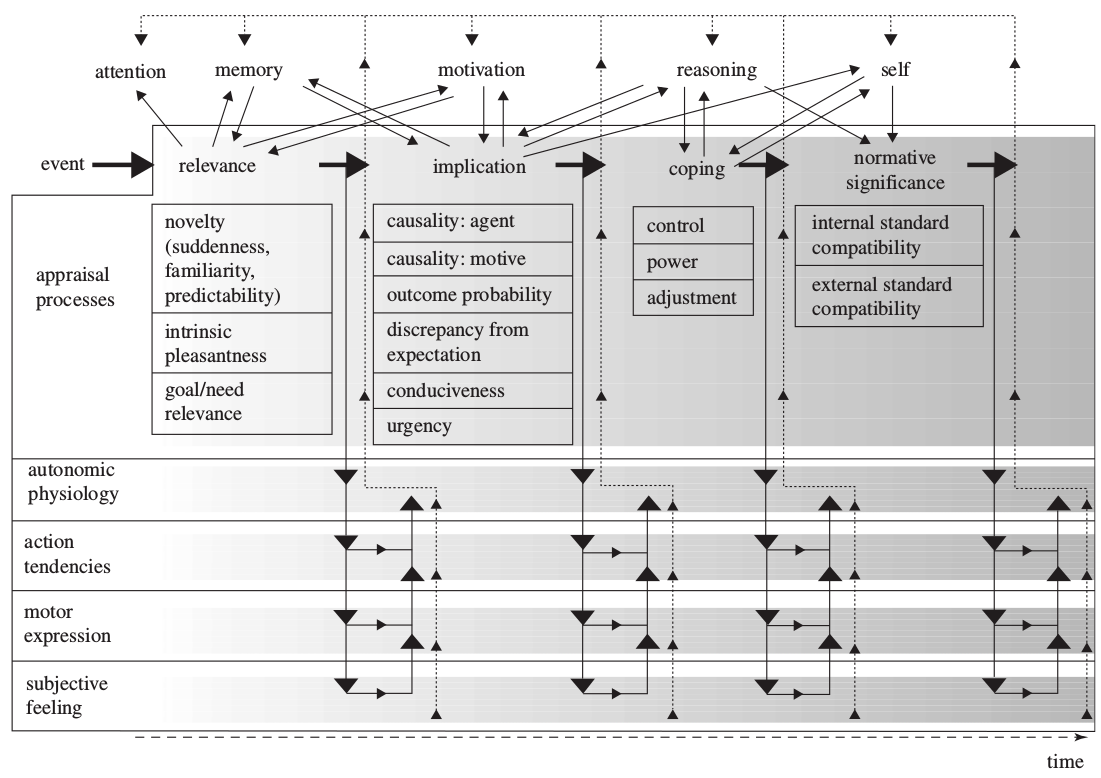
\includegraphics[width=\textwidth]{figure/comprehensive-CPM.png}
  \caption{Comprehensive illustration of the CPM of emotion
  \cite{scherer:dynamic-architecture-emotion,scherer:appraisal-processes}.}
  \label{fig:comp-cpm}
\end{figure}

\subsubsection{Appraisal Process}
\label{sec:appraisal-process}

According to this theory, appraisals are separable antecedents of emotion, that
is, the individual first evaluates the environment and then feels an appropriate
emotion \cite{scherer:appraisal-processes}. The appraisal procedure begins with
the evaluation process of the environment according to the internalized goals
and is based on systematic assessment of several elements
\cite{scherer:sequential-appraisal-process}. The outcome of this process
triggers the appropriate emotions. In many versions of the appraisal theory,
appraisals also trigger cognitive responses often called \textit{coping
strategies}. In fact, the coping mechanism manages the individual's action with
respect to the individual's emotional state and the existing internal and/or
external demands \cite{folkman:coping-pitfalls-promise}. The large majority of
computational models of emotions are based on this theory. An individual can
also use knowledge about the emotional reactions of others to make inferences
about them. According to the appraisal patterns, different emotions can be
experienced and expressed. Since expression of emotions reflects one's
intentions through the appraisal process, the \textit{reverse appraisal}
mechanism helps one to infer other's mental states based on their expressions.
\cite{gratch:reverse-appraisal, hareli:emotional-reaction-perception}.

Appraisal process is typically viewed as the cause of emotion and the cognitive
and behavioral changes associated with emotion. For instance, which particular
pattern of the appraisal variables (i.e., individual judgements) would elicit
certain emotion or an emotional expressions. These appraisal variables
include \cite{marsella:ema-process-model}:\\

\begin{itemize}
  \item \textbf{Relevance:} A relevant event has non-zero utility for an agent.
  This relevancy can either be based on negative influence of an event on the
  agent or a positive one.
  
  \item \textbf{Perspective:} The point of vierw in which an event will be
  judged, e.g. self or other.
  
  \item \textbf{Desirability:} A desirable event advances a state of the utility
  for an agent whose perspective is being taken, or inhibits that.
  
  \item \textbf{Likelihood:} A measure of likelihood of the outcome.
  
  \item \textbf{Expectedness:} The extent to which the truth value of a state
  could have been predicted from causal interpretation.
  
  \item \textbf{Causal Attribution:} The agent who desreves the credit/blame.
  
  \item \textbf{Controllability:} Whether the outcome can be altered by the
  agent whose perspective is taken (this variable is related to coping process).
  
  \item \textbf{Changeability:} Whether the outcome can be altered by some other
  causal agent (this variable is related to coping process).
\end{itemize}

Another key process invilved in appraisal is the coping process. This process
determines whether and how the agent shoud respond with respect to the outcome
of the appraising the events. There are several coping strategies that
computational models like EMA \cite{gratch:domain-independent} use as control
signals. These control signals enable or suppress the cognitive processes that
operate on the causal interpretation of the appraisal patterns. Coping process
controls the congruency of the acitons according to these patterns. As it is
shown below, in \cite{gratch:domain-independent} coping strategies are organized
into two categories of \textit{problem-focused} and \textit{emotion-focused}
coping strategies. Problem-focused coping strategies can be applied when the
agent requires to do something with respect to the problem, whereas
Emotion-focused coping works by changing one's interpretation of circumstances.
The following is a short list of a broad range of coping strategies
\cite{gratch:domain-independent}:

\begin{description}
  \item[Problem-focused coping] \hfill
	\begin{itemize}
	  \item \textbf{Active coping:} Taking active steps to remove or circumvent the
	  stressor,
	  \item \textbf{Planning:} Coming up w/ action strategies,
	  \item \textbf{Seeking social support for instrumental reasons:} Seeking
	  advice, assistance, or information.
	\end{itemize}
  \item[Emotion-focused coping] \hfill
    \begin{itemize}
	  \item \textbf{Seeking social support for instrumental reasons:} Getting
	  sympathy, moral support or understanding,
	  \item \textbf{Acceptance:} Accepting the stressor and learn to live with it,
	  \item \textbf{Restraint coping:} Waiting till the appropriate opportunity
	  (holding back).
	\end{itemize}
\end{description}

\subsubsection{OCC, a Structural Appraisal Theory of Emotion}

OCC model, similar to Lazarus' \cite{lazarus:cognitive-theory-emotion} and
Scherer's \cite{scherer:nature-function-emotion} cognitive views, considers
emotions to arise from affective or valenced reactions subsequent to the
appraisal of a stimulus as being beneficial or harmful to one’s concern
\cite{occ:structure}. The model categorizes emotions based on their underlying
appraisal patterns. These patterns are fundamental criteria a person employs for
evaluating the situation. They involve the person’s focus of attention, their
concern, and their appraisal preceding an affective reaction. Figure
\ref{fig:occ-model} shows main building blocks of OCC model.

\begin{figure}[tbh]
  \center
  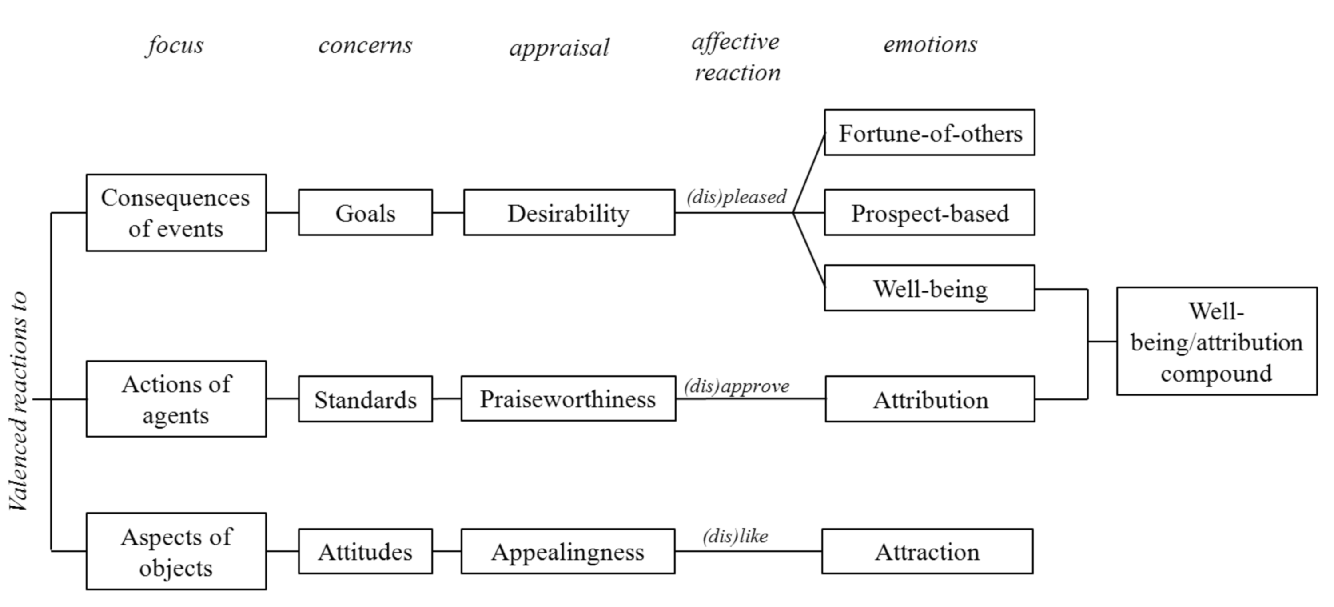
\includegraphics[width=\textwidth]{figure/occ.png}
  \caption{A simple visualization of OCC model \cite{occ:structure}.}
  \label{fig:occ-model}
\end{figure}

As shown in Figure \ref{fig:occ-model}, a person could alternatively have three
types of focuses. These types of focuses are consequence of events, actions of
agents, and aspects of objects. The person evaluates the significance of causes
behind these three types of focuses based on her personal concern. As a
result, an affective reaction will be elicited resulting in an emotion. Various
combinations of the elements depicted in Figure \ref{fig:occ-model} create
specific patterns demonstrating six main groups of emotions in which all emotion
types in a group share the same cognitive pattern. Emotion groups are
\textit{fortune-of-others, prospect-based, well-being, attribution,
well-being/attribution- compound}, and \textit{attraction}. The OCC model
introduces 22 emotion types. These emotions are introduced each as a
representative of a family of similar emotions with various intensities
(since relying on a list of discrete emotions that is understood by everyone
equally is impossible due to people's language barriers and various
interpretations of the actual words). For instance, happyness can be referred to
by other emotion terms such as joy, cheerful, glad, delighted while they all
share the same eliciting conditions. Thus the emotion types used in the model
(e.g., relief, love, pride, and shame) are meant to represent an emotional
experience rather than a lexical taxonomy.

Fo instance, as shown in Figure \ref{fig:occ-model}, the appraisal criterion for
consequences of event’s is their \textit{desirability} (see Section
\ref{sec:appraisal-theory}) for achieving one’s goals. This generates the
affective reaction of being \textit{pleased} in possitive cases, or
\textit{displeased} in negative ones. Figure \ref{fig:occ-structure} shows the
resulting emotion groups in OCC model such as \textit{fortune-of-others} (e.g.,
gloating, pity), \textit{prospect- based} (e.g., satisfaction, relief), and
\textit{well-being} (e.g., joy, distress) \cite{occ:structure}. The appraisal of
the praiseworthiness of the actions of an agent against one's personal
standards, as well as the appealing aspects of objects happens in the same way
as shown in Figure \ref{fig:occ-model}.

\begin{figure}[tbh]
  \center
  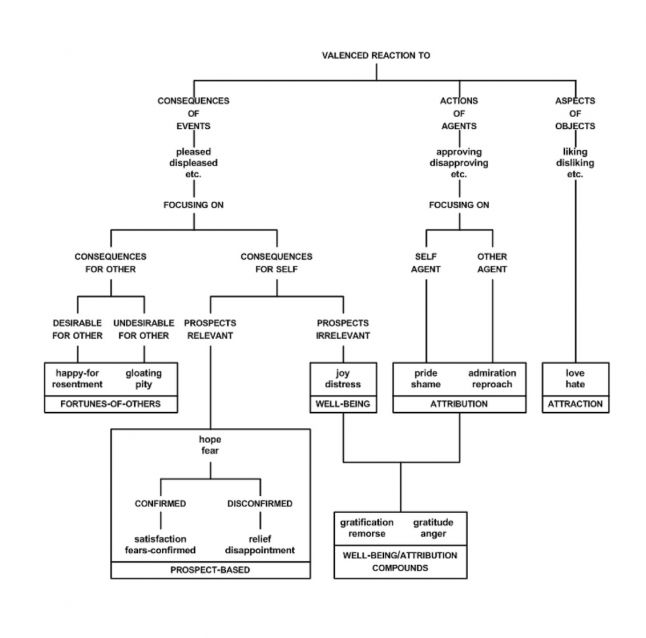
\includegraphics[width=0.9\textwidth]{figure/occ-structure.jpg}
  \caption{OCC taxonomy of emotion triggers and emotions \cite{occ:structure}.}
  \label{fig:occ-structure}
\end{figure}

Finally, the OCC model introduces some global variables of emotions intensity to
distinguish all types of emotions that a person could experience when
encountering events, agents or objects. These variables are as follows:

\begin{enumerate}
	\item Sense of reality (representing the degree to which the event, agent or
	object in focus appear real to the person),

	\item Proximity variable (representing the psychological proximity of event,
	agent or object),

	\item Unexpectedness (representing how unexpectedly one is taken by surprise,
	either positive or negative),

	\item Arousal (representing how arousing an event, agent or object is).
\end{enumerate}

\subsection{Constructivist (dimensional) emotion Theories}
\label{sec:dimensional-emotions}

The components and dimensions of emotions were the subject of much speculation
since the 19th century. Dimensional models of emotion attempt to conceptualize
human emotions by defining where they lie in two or three dimensions.
Dimensional theories of emotion argue that emotion should be conceptualized, as
points in a continuous (typically two or three) dimensional space rather than
looking at them as discrete entities (see Section \ref{sec:discrete-emotions})
\cite{carver:affect-behavior} \cite{mehrabian-russell:pad}
\cite{russell:core-affect} \cite{watson:consensual-structure-mood}. 

\begin{figure}[tbh]
  \center
  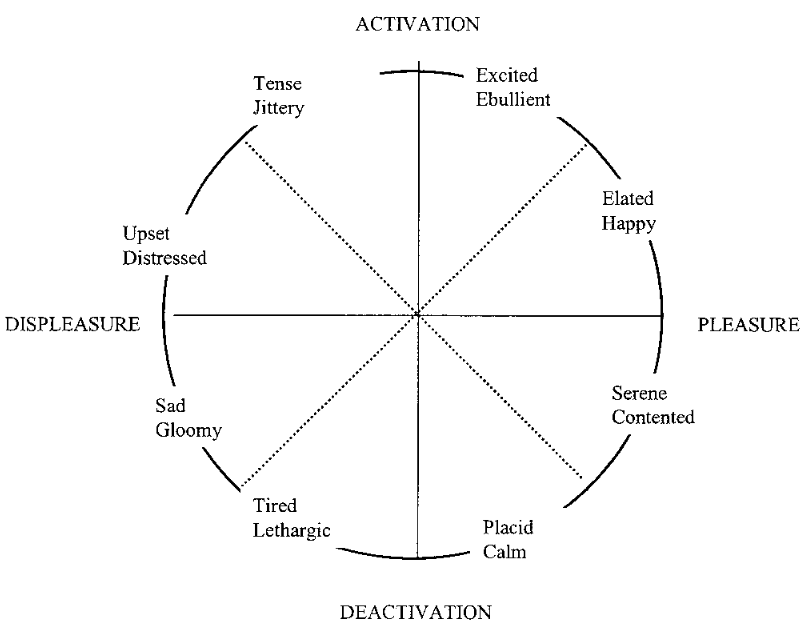
\includegraphics[width=.7\textwidth]{figure/core-affect.png}
  \caption{Core affect \cite{russell:core-affect}.}
  \label{fig:core-affect}
\end{figure}

Two dimensions that are commonly proposed to describe emotions are valence and
physiological arousal \cite{arnold:emotion-personality}
\cite{lazarus:cognitive-theory-emotion} \cite{russell:circumplex-affect}. Models
based on dimensional theories contrast theories of basic emotion, which propose
that different emotions arise from separate neural systems
\cite{posner:circumplex-affect}. Many dimensional theories argue that discrete
emotion categories (e.g., sadness, fear and anger) have no ``reality'' in that
there are no specific brain regions or functions that correspond to specific
emotions \cite{barrett:emotions-natural}. Dimensional theories do not emphasize
the term emotion.

\begin{figure}[tbh]
  \center
  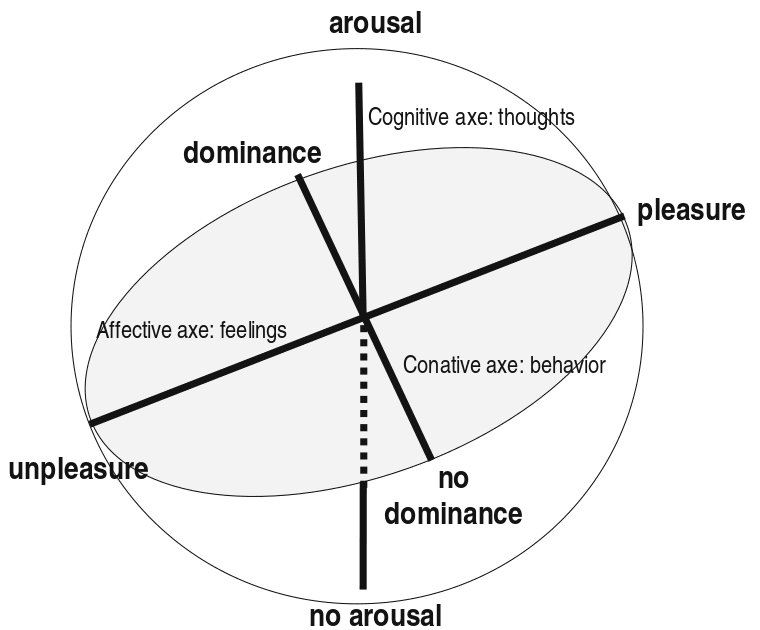
\includegraphics[width=.6\textwidth]{figure/dimensional2.png}
  \caption{Three dimensional model of pleasure, arousal and dominance as
  tripartite view of experience \cite{mehrabian:pad}.}
  \label{fig:pad}
\end{figure}

One of the two-dimensional models that are most prominent is Russell's
circumplex model \cite{russell:circumplex-affect}. Russell suggested that
affective states are all related to each other systematically through what is
called core affect \cite{russell:circumplex-affect,russell:core-affect} (see
Figure \ref{fig:core-affect}) and emotions are best described as a change in
core affect which, in turn, is describable as a point in a space between two
bipolar dimensions. One dimension is \textit{valence} or how good or bad are
objects and events for a being ranging from pleasant to unpleasant. The other
dimension is \textit{arousal}, ranging from calm to excited. Russell put a
number of affective states around a circular space between those two dimensions
(see Figure \ref{fig:core-affect}) which is also known as \textit{circumplex},
representing the variety of core affects
\cite{russell:circumplex-affect,russell:core-affect}. Since sometimes
two-dimensional space cannot easily differentiate among emotions that share the
same values of arousal and valence, e.g., anger and fear (both characterized by
high arousal and negative valence), some of the dimensional models incorporate
valence and arousal as well as \textit{intensity}, or \textit{dominance}
or stance dimensions. Many computational dimensional models build on the three
dimensional “PAD” model of Mehrabian and Russell \cite{mehrabian-russell:pad}
where these dimensions correspond to pleasure (a measure of valence), arousal
(indicating the level of affective activation) and dominance (a measure of power
or control). Figure \ref{fig:pad} shows these three dimensions.

\begin{figure}[tbh]
  \center
  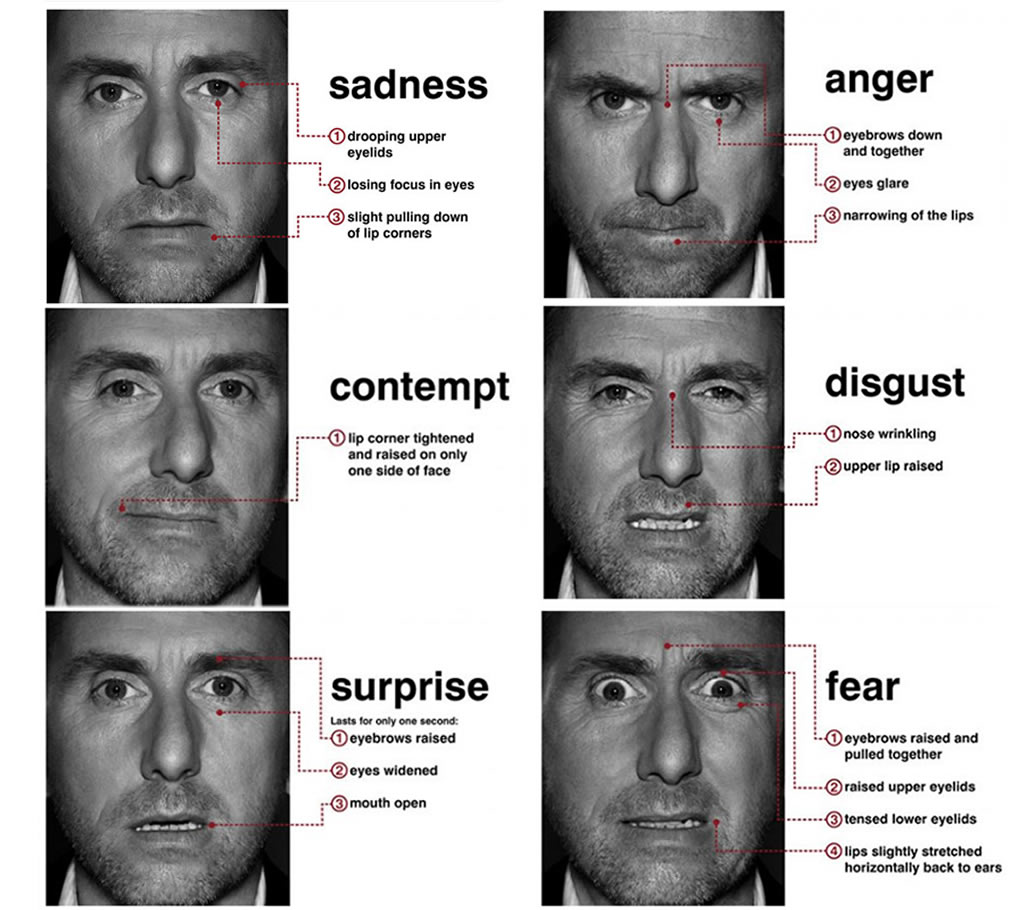
\includegraphics[width=.9\textwidth]{figure/basic-emotions.jpg}
  \caption{Basic emotions and corresponding expressions.}
  \label{fig:basic-emotions}
\end{figure}

\subsection{Basic (discrete) emotion theories}
\label{sec:discrete-emotions}

Basic emotion theories are inspired by Tomkins' \cite{tomkins:affect}
rediscovery of Darwin's work
\cite{darwin:emotion-expression,hess:darwin-emotion} which later were developed
by Ekamn \cite{ekman:argument-emotions} and Izard \cite{izard:human-emotions}.
These theories emphasize a small set of discrete and fundamental emotions.
The underlying assumption of this approach is that these emotions are mediated
by associated neural circuitry, with hardwired component
\cite{ekman:argument-emotions}. Different emotions are then characterized by
stable patterns of triggers, behavioral expression, and associated distinct
subjective experiences. The emotions addressed by these theories are typically
called the \textit{basic} emotions. Emotions including happiness, sadness, fear,
anger, surprise, and disgust are often considered to comprise the most
prototypical basic emotions \cite{ekman:argument-emotions}. The theory of basic
emotions holds that there is a set of emotions shared by all humans that evolved
to deal with ancestral life challenges \cite{ekman:argument-emotions}. For
instance, disgust evolved to deal with the challenge of avoiding noxious
stimuli, and fear evolved to deal with the challenge of avoiding dangers.
Because of the emphasis on discrete categories of states, this approach is also
termed the \textit{categorical} approach \cite{panskepp:affective-neuroscience}.
Much of the supporting evidence offered for the theory comes from experiments
that show how certain facial expressions are universally associated with
specific basic emotions, regardless of the observer's cultural background. This
universality has a production side and a recognition side. On the production
side, a particular emotional state is said to elicit a facial expression
comprised of a fixed set of facial muscles. On the recognition side, observers
are able to infer the emotional state of the person who expresses an emotion,
due to the direct correspondence between emotional states and the facial
expressions they cause. Computational models inspired by the basic emotions or
discrete approach often focus on low-level perceptual-motor tasks and encode a
two-process view of emotion that argues for a fast, automatic, undifferentiated
emotional response and a slower, more differentiated response that relies on
higher level reasoning processes (e.g.,
\cite{armony:computational-modeling-emotion}).

\subsection{Other Approaches}

\subsubsection{Rational Approaches}

Rational approaches start from the question of what adaptive function does
emotion serve and then attempt to incorporate these functions into a model of
intelligence. Emotion, within this approach, is simply another set of processes
and constraints that have adaptive value. Models of this sort are most naturally
directed towards the goal of improving theories of machine intelligence
\cite{anderson:newell-cognition} \cite{scheutz:affect-agent}
\cite{simon:motivation-emotion-cognition}.

\subsubsection{Communicative Approaches}

Communicative theories of emotion argue that emotion processes function as a
communicative system. They can function first, as a mechanism for informing
other individuals of one’s mental state (thereby facilitate social
coordination), and second, as a mechanism for requesting/demanding changes in
the behavior of others. Communicative theories emphasize the
social-communicative function of expressions \cite{gratch:emotion-intention}.
Computational models inspired by communicative theories focus on machinery that
decides when an emotional expression can have a desirable effect on a human
counterpart.

\section{Relation to Psychology and Sociology}

- Refer to functions of emotions (Page 48 in proposal).

\subsection{Emotion in Social Context}

Emotions are involved in developing social context. Humans are social and most
of the causations and constitutions of their emotions are social. Brian
Parkinson in \cite{parkinson:emotions-social} argues that many of the causes of
emotions are interpersonal and communicative rather than internal and reactive
phenomena. There are different social aspects of emotions influenced by various
factors such as social context and social relationship type. For instance, a
dominant-submissive social relationship can cause and contain different emotions
with different intensities compared to a reciprocal or a friendship social
relationship type. As another example, an emotion can be interpreted in a
certain way when an individual is situated in an environment with other people
who are expressing a particular emotion.

There are numerous ways that emotions can be
social \cite{tiedens:social-life}. There is a consensus on the fact that social
events and entities surrounding the individual play an essential role in the
generation of emotion. There are several ways in which other people elicit
emotional responses in us. One is that we feel the emotions of those around us.
Also, we have emotions about actions of those people around us. Another is we
have emotions about the things that happen to other people. Yet another is our
concern about our relationship with others that elicits emotion in us. The
groups to which we belong can also elicit our emotions. Moreover, we can feel
emotion about the success and failure of our own group or of other groups. In
addition, groups or individuals may make salient cultural concerns or societal
expectations that can elicit our emotions.

Beside the fact that social context can cause eliciting emotions in individuals,
social context provides information about what emotion should be expressed, by
whom, and in what situations. For instance, people are well aware of the
inappropriateness of expressing too much emotion to acquaintances
\cite{tiedens:social-life}. However, the social knowledge of emotion expression
is only partially delivered in an explicit fashion. There are studies on the
regulatory role of society and social relationships on emotions, showing that
people's emotions become socialized in implicit and unconscious ways. From this
perspective, social context can control and direct our attention toward certain
types of events and away from others.

\subsection{Social Meaning of Events}

Humans are emotional and social beings. Their emotions and the social context
in which they are involved have mutual impacts on each other. But, what if
humans can share their emotions with others just as they share their thoughts,
resources and their environment. Sharing an emotion with others may alter the
experience of an event. For instance, according to the nature of the
relationship between the individuals, the expression of emotions can either
restrain them from further interactions or improve their relationship.
Furthermore, individuals sharing emotions might possess a shared understanding
of their environment. Socially shared and regulated emotions also provide social
meanings to the events happening in the environment
\cite{wisecup:sociology-emotions}. For instance, people are likely to make
social inferences based on the presence or absence of particular emotions in
their social environment. Moreover, emotions can provide a basis for judgment
depending on the individual's relationships with others. In other words,
emotions can associate or disassociate an individual, therefore, they can change
or maintain the individual's social relationships \cite{tiedens:social-life}.

\subsection{Social Motivator}

Emotions can also play the role of a motivator in a social context. There is a
subset of social emotions delineated as role-taking emotions in
\cite{shott:emotion-social-life}. Shott provides two categories of
\textit{reflexive} (e.g. shame or pride) and \textit{empathic} (e.g., empathy or
pity) role-taking emotions. The reflexive emotions can motivate the individual's
self-control which depends on the anticipated reactions of others to the
individual's behaviors. For instance, guilt might lead the individual to behave
altruistically to restore a positive social stance for that individual. Empathic
or vicarious emotions are based on an individual mentally placing himself in
other's situation to understand how the other feels in that situation. These
emotions motivate prosocial behaviors to maintain an individual's internal
well-being \cite{thoits:socialogy-emotion}.

\subsection{Communicating Emotions}

Humans need to communicate their emotions within the social context
for different reasons. In \cite{goffman:self-presentation} Goffman argues that
human behaviors around others are performative which is often intended to convey
information to others. When human's actions are visible in the social context,
they behave differently in the presence of the others
\cite{zajonc:social-facilitation}. The social life of an individual is comprised
of the individual's internal cognitive competencies and his interactions in the
society. Lazarus says, if society is a fabric, then emotion is its color
\cite{lazarus:emotion-adaptation}. Although emotions undeniably have personal
aspects, they are usually experienced in a social context and acquire their
significance in relation to this context
\cite{parkinson:emotion-social-interaction}.

A successful and effective emotional communication necessitates ongoing
reciprocal adjustments between interactants that can happen by interpreting each
other's behaviors \cite{parkinson:emotion-social-interaction}. It not only
requires proper interpretation of the other's expressions, but also correct
assessment of the extent to which others can read an individual's expressions.
In emotional communication, individuals are constantly exchanging messages about
their mental states, and modifying each other's emotional responses as they
occur. Individuals perceive other's emotional states through verbal and
nonverbal responses during the interaction by processing relevant messages.
Communication dynamics represent the temporal relationship between these
communicative messages. The verbal and nonverbal messages from one participant
are better interpreted inside the correct context including the history and the
ongoing messages from the other individuals. Interpersonal dynamics (also known
as micro-dynamics in sociology) represent this influence of relationships
between individuals \cite{louis:communication-dynamic}.

\subsection{Social Functions}

Humans are able to communnicate their emotions in a social context. The social
functions of emotions are the reason behind why humans try to communicate their
emotions. In this section, I briefly discuss these social functions of emotions
since they are directly related to my work. Ekman in
\cite{ekman:argument-emotions} asserts that the primary function of emotions is
to mobilize the organism to deal with important interpersonal encounters. Darwin
in \cite{darwin:emotion-expression} argues the significance of social
communicative functions of emotions. Emotions describe interpersonal dynamics in
a way that they can constitute individuals' relationships
\cite{parkinson:emotions-social, tiedens:social-life}. One aspect of expressing
and communicating emotion in a social context is to express one's social motives
and intentions \cite{hess:darwin-emotion}. Another aspect of communicating
emotions is to reveal the underlying mental states of an individual
\cite{parkinson:emotion-communication}. In other words, emotions constitute two
different functionalities of expressing communicative signals associated with
one's social motives and intentions as well as expressing one's internal states
and how one feels about something. In \cite{kleef:emotion-regulate-social} Van
Kleef has discussed the idea of inferential processes with which individuals can
infer information about others' feelings, relational orientations and behavioral
intentions based on their emotional expressions. He also argues that emotional
expressions can impact social interactions by eliciting others' affective
responses.

Functional accounts vary according to the kind of system being analyzed.
Therefore, functional approaches to the emotions should vary by level of
analysis. Social functions of emotions can be analyzed in \textit{individual,
dyadic, group} and \textit{cultural} levels. My focus in this research is
on social functions in dyadic interaction (more specifically collaboration); I
also consider these functions at the individual's level especially when
interpreting the other collaborator's behaviors. Studies in all these levels
share a few assumptions about social accounts of emotions. They assume a)
individuals are social by nature and pursue solutions to survival problems in
social relationships, b) individuals apply their emotions to coordinate their
social interactions and relationships to address these survival problems, c)
emotions are processes mediating the individuals' relations to their dynamic
environment \cite{keltner:emotion-functions}. In dyadic interactions, studies
focus on how emotions impact the interactions of individuals in meaningful
relationships. In \cite{keltner:emotion-functions} Keltner and Haidt discuss
that in a dyadic setting, researchers mostly focus on communication of emotion
(e.g.\,Scherer \cite{scherer:vocal-expression}, DePaulo
\cite{depaulo:nonverbal-behavior}), properties (e.g.\,emotion contingency,
emotion synchrony) of dyadic emotions (e.g.\,Levenson \& Gottman
\cite{levenson:affective-exchange}), discourse (e.g.\,Bretherton
\cite{bretherton:emotions-functionalist}), and attachments (e.g. Hazan \& Shaver
\cite{hazan:emotion-attachment}).

\subsection{Dyadic Interaction}

As mentioned earlier, the social context is an important factor influencing
one's emotions. A dyadic interaction is one type of a setting in a social
context. Dyadic interaction tasks allow us to study emotion in a social setting
\cite{coan:emotion-dyadic}. Dyadic interaction tasks make it possible to examine
how individuals experience and express emotions during social interactions and
how emotions shape and are shaped by the reciprocal interactions between
individuals. In addition, eliciting and monitoring emotional processes yields
useful information about the role emotion plays in interpersonal relationships.
Compared with other emotion-eliciting events, events in a dyadic interaction can
better help us study an ongoing emotional relationship between two individuals
in addition to their internal emotional and cognitive processes. Dyadic
interaction tasks are ideal for studying a range of emotional responses because
of the fairly unstructured conversations between the individuals. Thus, dyadic
interaction tasks will generate a wide range of emotions in comparison with the
controlled emotion-eliciting events.

\section{Similarities and Differences}

Different theoretical perspectives should not be viewed as competing for a
single ground truth. They should be seen as distinct perspectives, each arising
from a particular research area (e.g., biological vs. social psychology),
focusing on different sets of affective phenomena, considering distinct levels
of resolution and fundamental components (e.g., emotions vs. appraisal variables
as the distinct primitives). These different perspectives also provide different
degrees of support for the distinct processes of emotion, e.g., the componential
theories provide extensive details about cognitive appraisals
\cite{hudlicka:guidelines-emotions}. Therefore, I am going to provide a
pairwise comparison between these fundamental theories.

\subsection{Dimensional Vs. Discrete (Basic) Emotion Theories}

The fundamental assumption of the basic emotion theory is that a specific type
of event triggers a specific affect programme corresponding to one of the basic
emotions and producing characteristic expression patterns and physiological
response configurations \cite{scherer:emotions-emergent}. Dimensional theory's
main criticism of basic emotions theory is based on the observation that
affective phenomena appear to be both qualitatively and quantitatively diverse.

Russell in \cite{russell:core-affect} argues the labels such as ``fear",
``anger'', ``happiness'' do not capture this diversity. For instance, one might
say: a) a person being chased by an assailant brandishing a knife, b) a person
who retreats from an insect moving across the floor, and c) a person who is
concerned they will never find a career that is fulfilling are all in a state of
fear. On the basic emotions account, an emotional episode involves fixed
patterns of neurophysiological and facial expression changes in response to an
eliciting stimulus that are distinct between emotions, but are the same within
the same emotional category \cite{ekman:argument-emotions}. If this were the
case, one would expect that the three individuals described above would respond
to their eliciting stimuli in the same way, yet the similarity of behavioral
responses between these three cases seem unlikely. Dimensional theorists, in
contrast, would argue that the individuals in the above three cases are applying
the concept of fear to experience, despite the fact that each individual has a
unique core affect. While basic emotion theorists would hold that since all
three individuals are experiencing fear, they would perform the same behavioral
responses to the stimuli, dimensional theorists would argue this is not the
case, as each individual bears a core affective state that is distinguished from
the other two. For instance, the individual's arousal in response to an armed
assailant should be higher than the individual in response to an insect, as the
former case poses a threat to their life. As a result, the individual in the
first case would likely make every effort to escape from the assailant,
including trying to negotiate and plead with the assailant, while the individual
in the second case would be relatively less dedicated to escaping the insect. 

In sum, dimensional theory is compatible with the differences in the behavioral
responses to eliciting stimuli, while basic emotions theory only allows for a
single fixed behavior of responses to a given emotion. Furthermore, dimensional
theories can represent instances of basic emotions (see Figure
\ref{fig:dimensional-discrete}), for example, fear elicited by a snake (green
rectangle), in terms of variation along affective dimensions, i.e., arousal and
valence.

\begin{figure}[tbh]
  \center
  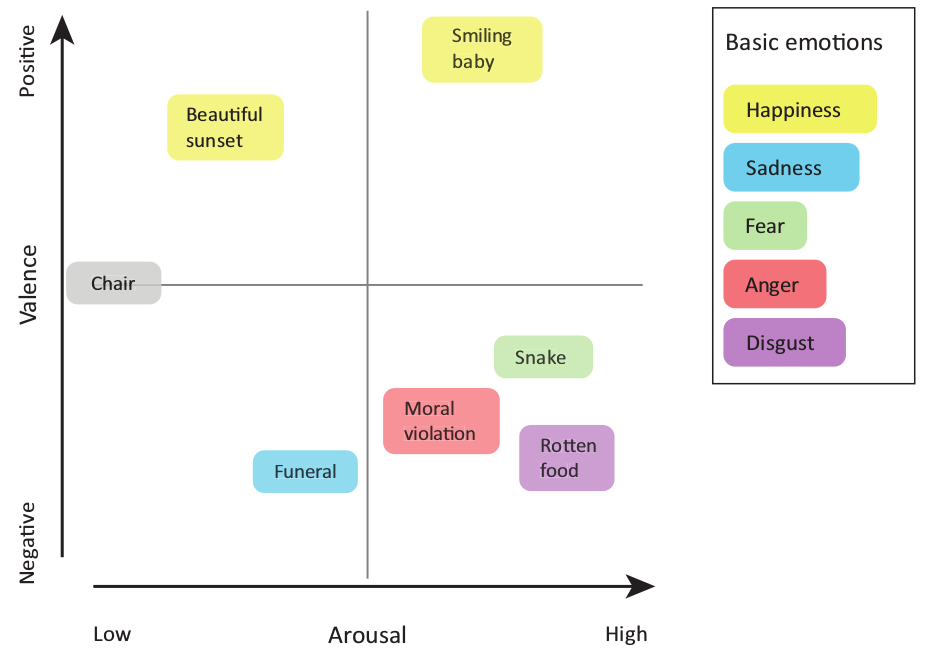
\includegraphics[width=.9\textwidth]{figure/dimensional-discrete.png}
  \caption{Representing basic emotions within a dimensional framework
  \cite{hamann:mapping-discrete-dimensional}.}
  \label{fig:dimensional-discrete}
\end{figure}

Also, basic emotion theory fails to account for affect that lacks
object-directedness \cite{russell:core-affect}. In basic emotions approach, an
emotion is supposed to have an intentional object it is directed towards (e.g.,
being angry at someone, or being sad for someone). The dimensional theory argues
that emotion may not necessarily be aimed at a particular object. For instance,
an individual can experience a certain type of emotion (e.g., anger) without
knowing of anything in particular that has offended them. Dimensional models of
emotion are therefore capable of accounting for a wider range of affective
phenomena than basic emotions theory.

Another difference between dimensional and basic emotion theories is that the
basic emotion categorization of emotions captures facets of the experience of
an emotion not conveyed by the dimensional description, such as elicitation of a
facial expression of the emotion. In fact, this attribute of the basic
emotions theory is one of the major differnces with all other emotion theories.
As it is argued in basic emotion theory, basic emotions are hard-wired to their
corresponding facial expressions. Ekman who elaborated the concept of basic
emotions, developed the \textit{Facial Action Coding System} (FACS) which
encodes movements of individual facial muscles and it is a common standard to
systematically categorize the physical expression of emotions
\cite{ekman:facial-movement}.

\subsection{Appraisal Vs. Dimensional Emotions Theories}

Dimensional theories might suffer to adequately distinguish emotions because
of the existance of the limited dimensions.

To compare the appraisal and dimensional theories of emotion, we can argue that
there is a relationship between the dimensions in the constructivist or
dimensional theory of emotion and appraisal dimensions. For instance, the
pleasure dimension roughly maps onto appraisal dimensions that characterize the
valence of an appraisal-eliciting event (e.g., intrinsic pleasantness
--desirability--, or goal congruence), dominance roughly maps onto the appraisal
dimension of coping potential, and arousal can be considered as a measure of
intensity. However, they also have quite different meanings. Appraisal (as I
mentioned earlier) is a relational construct characterizing the relationship
between some specific object/event in the environment and the individual's
mentals constructs including beliefs, motives and intentions and several
appraisals may be simultaneously active; whereas emotions in dimensional emotion
theory are non-relational constructs, each summarizing a unique overall state of
the individual.

Furthermore, dimensional emotion theories emphasize different components of
emotion than appraisal theories and link these components quite differently.
In contrast to appraisal theories, dimensional emotion theories do not address
affect’s antecedents in detail. However, dimensional theorists question the
tight causal linkage between appraisal and emotion that is central to appraisal
accounts. As mentioned earlier, dimensional theorists believe that the emotion
is not necessarily about some object (as in ``I am angry \underline{at him}'').
In such theories, many factors may contribute to a change in emotion including
intentional judgments (e.g., appraisal). However, in dimensional emotion
theories the link between any preceding intentional meaning and emotion is
broken and most of the time can not be recovered correctly. For example, Russell
argues for the following sequence of emotional components: some external event
occurs (e.g., a bear walks out of the forest), it is perceived in terms of its
affective quality; this perception results in a cruicial change in core affect;
this change is attributed to some ``object" (e.g., the bear); and only then is
the object cognitively appraised in terms of its goal relevance, causal
antecedents and future prospects \cite{marsella:computational-models}.

We can also compare the dimensional emotion theories to OCC model as cognitive
appraisal model. The major similarity between these two models is that they both
consider emotions to descend from valenced reactions to the stimuli.
Furthermore, they acknowledge the role of arousal in determining emotional
reactions. As we mentioned in Section \ref{sec:dimensional-emotions} Russell
considered arousal as one of the two key dimensions of emotions which could be
used to partially discriminate emotional states
\cite{russell:circumplex-affect}. In a different manner, the OCC model
recognizes arousal as a necessary condition for eliciting emotions, and regards
the arousal as a major determinant of emotion’s intensity which distinguishes
among various emotions of a particular type (e.g., fearful and scared). In
\cite{scherer:what-emotions} Scherer speculates that arousal dimension in
dimensional models gives little information about the underlying appraisal of
the elicited emotion and he proposes to replace it with coping potential which
is an appraisal dimension referring to individual’s perceived control in a given
situation. 

Furthermore, models based on dimensional emotions theory pursue the idea of
eliciting an emotion according to the joint features in circumplex space (2D or
3D -- see Section \ref{sec:dimensional-emotions}) while OCC or other
models of appraisal theory are based on patterns of antecedent of emotions. This
is the fundamental difference between OCC, or appraisal theories in general, and the
circumplex approach of Russell \cite{russell:circumplex-affect} or Mehrabian's
PAD model \cite{mehrabian:pad,mehrabian-russell:pad}. Also, models based on
appraisal theory of emotion employ causation, attribution and eliciting
conditions in order to distinguish emotions while the eliciting conditions are
not directly accessible from dimensional approach. A dimensional model might
fall short in establishing why certain emotions are elicited. However, when the
objective is to identify the generated emotions and their level of pleasantness
and intensity, circumplex model brings about a perfect opportunity
\cite{ahmadpour:occ-dimensional-comparison}.

Finally, here, I discuss how a model based on dimensional emotions theory
(i.e., Russell's 2D circumplex) relates to a cognitive model based on appraisal
theory (i.e., OCC model). Figure \ref{fig:occ-circumplex} shows the relationship
between Russell's circumplex and OCC model in terms of categorization of the
actual emotions. The number of emotions in a section of Russell's circumplex
that fall into an emotion group of OCC are shown in parentheses (see Figure
\ref{fig:occ-circumplex}). For instance, all three emotions on the top section
(highly excited, neutrally valenced emotions) fall into prospect based emotion
group, hence number (3) is indicated. Or, as another example, emotions in the
left section (neutral arousal value, negative valenced emotions) make a one to
one relationship between disappointment and prospect based emotion group,
contempt and attribution emotion group, and jealousy and fortune of others
emotion group, hence number (1) is indicated in fornt of each.

\begin{figure}[tbh]
  \center
  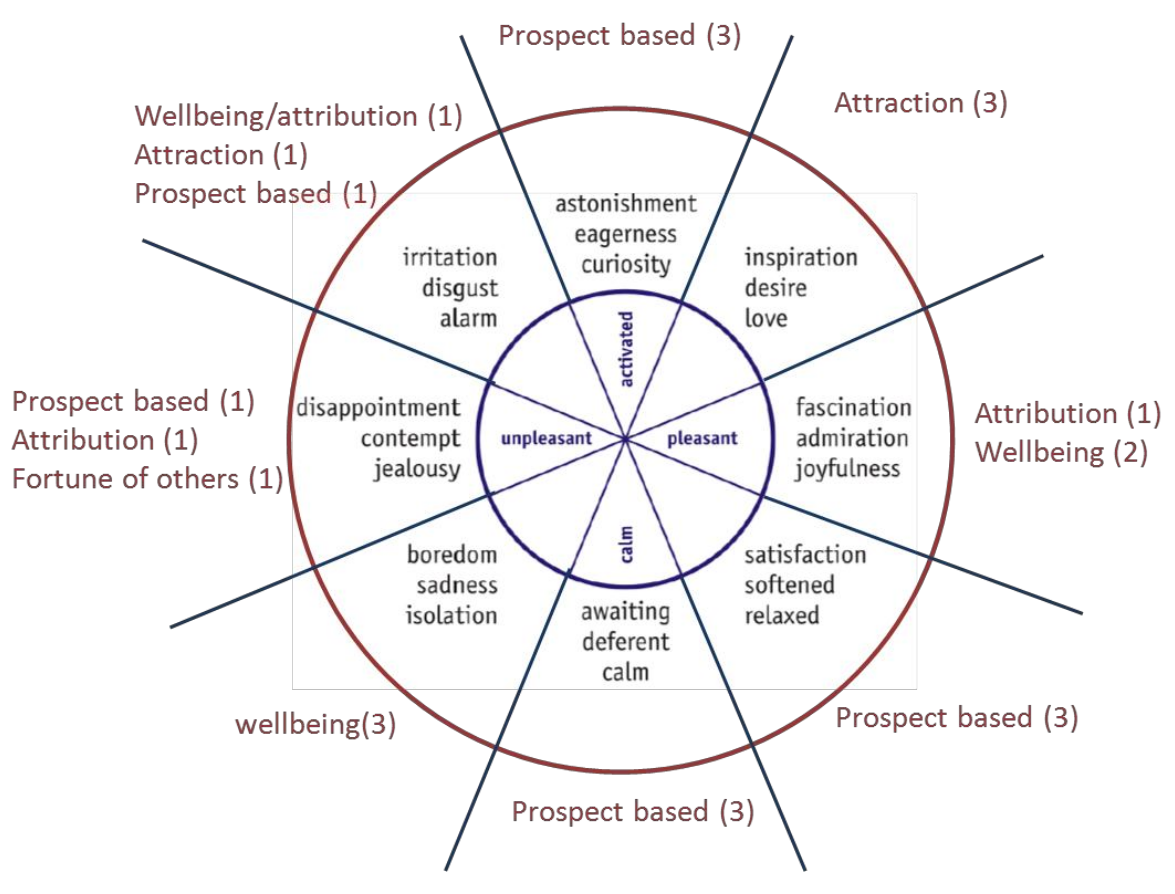
\includegraphics[width=.9\textwidth]{figure/occ-circumplex-mapping.png}
  \caption{A rough projection of emotion groups of OCC on the circumplex of
  affect \cite{ahmadpour:occ-dimensional-comparison}.}
  \label{fig:occ-circumplex}
\end{figure}

\section{Applications in Autonomous Agents and Robots}

There are several examples in artificial intelligence and robotics of applying
the appraisal theory as the basis of a computational model for emotions
\cite{adam:bdi-emotional-companion,kim:model-hri-appraisal,
marsella:ema-process-model}. In \cite{sander:systems-approach-appraisal} authors
describe a system approach to appraisal processes based on Scherer's work on
appraisal and the Component Process Model (CPM)
\cite{scherer:nature-function-emotion}. They show how the temporal unfolding
of emotions can be experimentally tested. In this thesis, I use the cognitive
appraisal theory of emotion provided by Gratch and Marsella in
\cite{gratch:domain-independent}. They lay out a general domain-independent
computational model of appraisal and coping. I use this appraisal approach,
in general, as an evaluation mechanism for the internal and external events to
assist the cognition and collaboration processes in my theory.

- Rewrite this [Computational dimensional models are most often used for
animated character behavior generation, perhaps because it translates emotion
into a small number of continuous dimensions that can be readily mapped to
continuous features of behavior such as the spatial extent of a gesture. For
example, PAD models describe all behavior in terms of only three dimensions
whereas modelers using appraisal models must either associate behaviors with a
larger number of appraisal dimensions (see Scherer and Ellgring, 2007, Smith and
Scott, 1997) or map appraisals into a small number of discrete, though perhaps
intensity-varying, expressions (Elliott, 1992). For a similar reason,
dimensional models also frequently used as a good representational framework for
systems that attempt to recognize human emotional behavior and there is some
evidence that they may better discriminate user affective states than approaches
that rely on discrete labels (Barrett, 2006).]

\subsection{Sociability}
Social skills have been mostly neglected in artificial intelligence and
robotics. However, there is a broad discussion in natural and social sciences,
e.g. psychology and primatology \cite{beheshtifar:social-intelligence-leadership,
bradberry:ability-skill-intelligence, keating:search-social-intelligence,
wexler:emotional-intelligence-appraisal, worden:primate-social-intelligence},
about the role of social factors in the development of intelligence
\cite{dautenhahn:social-autonomous-robots} (see Sections
\ref{section-emotion-social} to \ref{section-emotion-social-functions}). Robots
in the real world, e.g. domestic robots or collaborative robots, require
extensive understanding of aspects of humans' behaviors within their environment
as well as the ability to communicate and collaborate with them. Emotions, as
coordinated responses to detected or inferred relational meanings of the
environment (based on appraisal theory), can provide understanding of the social
environment, and the capability of communicating internal mental states and
maintaining collaborations with human partners. In fact, the emotion processes
momentarily respond to the unfolding affordances and constraints offered by the
dynamic context of a social interaction \cite{parkinson:holds-emotion}.
Appraisal can provide the assessment of goal relevance and goal congruence with
focus on self or other, the event, or the object in a social context
\cite{parrott:appraisal-social-emotions}. In short, the agent will be capable of
appraising the social environment in order to maintain effective social
interaction.

\subsection{Decision Making}

Decision-Making is an important and complicated process for any robot or virtual
agent. This process becomes more complicated when the agent needs to make a
decision considering its own private goal, the collaboration's shared goal and
the human collaborator's interests. I will provide more details about the
following concepts in Chapter \ref{chapter-theory}.

There are examples of rational and social agents designed based on the decision
theory and emotional states \cite{gmytrasiewicz:emotion-agent-decision}. Agents
must take a form of action after making a decision. Zhu and Thagard argue how
emotions significantly affect the action generation procedure as well as action
execution and control \cite{zhu:emotion-action}. The decision-making procedure,
as the basis of an agent's behaviors and actions, is a crucial process for an
agent in a social environment. Decision-making is a process that unfolds over
time and should be explored in more detail. According to
\cite{paulus:emotion-decision-belief}, the temporal structure of the
decision-making process contains three component processes:

\begin{enumerate}
  \item Choosing among options initially involves the process of
  \emph{assessing} the available options. One's affective state and appraisal
  evaluation of one's internal state as well as the surrounding environment
  helps in the assessment of all available options. For example, based on the
  scenario in section \ref{example-scenario}, Robot's emotion instance is fear
  because of an existing block in the plan and its evaluation of Astronaut's
  emotion as anger (for the same reason). The assessment of available options
  will be based on minimizing the distance to the shared goal and Astronaut's
  satisfaction. For instance, if Robot faces a non-critical task, it will give
  higher value to Astronaut's demanding task which will cause the postponement
  of its own.
  
  \item This process is followed by the \emph{selection} of an option based on
  the value that has been assigned to the option. This process is also augmented
  by affective evaluation of the world, including self, other(s) and the
  environment. For instance, in our scenario (see section
  \ref{example-scenario}), following the assessment of available options, Robot
  will focus on Astronaut's preferred task. Also, Robot creates and annotates
  meta information of the current state of the collaboration with affective
  evaluations.
  
  \item Finally, the outcome associated with the selected action is
  \emph{evaluated} and \emph{incorporated} into existing knowledge for
  subsequent decisions which implicitly and explicitly help the belief and
  appraisal emotion systems to operate coherently over time. For instance, if
  something goes wrong the Robot gives a negative affective attribution to the
  outcome of the selected action or even a certain path to that action to be
  used in future assessments.
\end{enumerate}

People's experience of events leak into their beliefs and ultimately decisions.
One aspect of these type of experiences is conscious or unconscious annotations
by different emotions. For instance, one will never forget working with a friend
due to the pleasant feeling of experiencing the outcome. On the other hand, a
person will always remember a particular experience in life because of an
utterly negative emotion that was felt at the time
\cite{paulus:emotion-decision-belief}.

Emotions appear to influence the value and weight computation of available
alternatives, and these computations are dynamically adjusted based on the
environment and the individual's internal states
\cite{pomerol:ai-decision-making}. This way agents can operate and take actions
based on preferences. In other words, emotional states of individuals are linked
to their decision-making processes, assuming that emotions affect the way gains
or losses are transformed to weights and values of the alternative beliefs,
actions, tasks, and, in general, plans \cite{paulus:emotion-decision-belief}.
The outcome of an action is also profoundly bound to the decision making process
as a final and an important stage. The experience of an outcome and in
particular, the differences between the expected and observed outcome provides
an opportunity to improve one's beliefs about consequences (value) of the
available alternatives and adopt a better decision policy in the future
\cite{pomerol:ai-decision-making, paulus:emotion-decision-belief}.

\section{Conclusion}

\bibliographystyle{plain}
\bibliography{mshayganfar}

\end{document}
